\chapter{Avaliação exploratória}

\section{Cenário-tipo selecionado}

%explicar qual foi o cenário selecionado para experimentar em cada plataforma (deve ser uma parte dos requisitos gerais do capítulo 3)
Antes de avançar com o desenvolvimento do sistema foi necessário escolher um backend para dar suporte tanto à aplicação móvel, como à aplicação web. Para isso foi desenvolvido um cenário idêntico com ambos os backends em que pudéssemos fazer uma análise comparativa dos pontos fortes e ou fracos entre eles. \par 
O cenário escolhido para esta avaliação exploratória foi o simples ato de recolher a frequência cardíaca do sensor do \gls{VJ} e guardar no backend em estudo, para posteriormente visualizar um simples histórico dos dados inseridos. Na figura \ref{f:study-overview} temos uma simples visão das várias partes envolvidas nesta avaliação.

\begin{figure}[H]
  \centering
  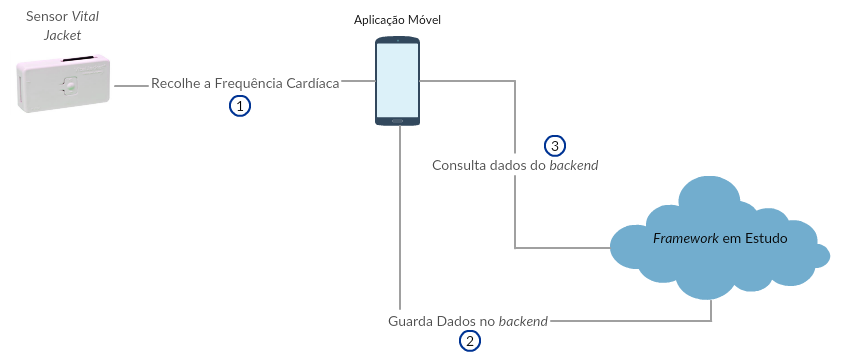
\includegraphics[width=0.9\textwidth]{imgs/study-overview.png}
  \caption[Diagrama geral do cenário de estudo]{Diagrama geral do cenário de estudo}
  
  \label{f:study-overview}
\end{figure}

A escolha de um backend para a solução era um ponto importante. Das várias frameworks disponíveis para um possível backend foram selecionadas três para ser desenvolvido o cenário com o objetivo de concluir se seria uma boa hipótese para a solução, entre elas estão: \gls{OMH}, \gls{FHIR} e Google Fit. \par

Para utilizar cada uma destas frameworks, foi desenvolvida uma aplicação móvel, bastante simples, a aplicação móvel tinha várias funcionalidades. Entre elas temos:
\begin{itemize}
  \item Seleccionar o dispositivo com os sensores
  \item Efetuar Login na respetiva framework
  \item Guardar leituras de frequência cardíaca num determinado segundo
  \item Visualizar as leituras inseridas
\end{itemize}

Tendo em conta que a mesma aplicação conseguia utilizar os três backends distintos, esta seleção era feita tendo em conta o tipo de login efetuado.


\section{Implementação exploratória: Open mHealth}
%http://www.openmhealth.org/documentation/#/store-data/storage-overview
%http://projects.spring.io/spring-security-oauth/docs/oauth2.html
%explicar a implementação que foi feita para esta tecnologia, dificuldades, adaptações, "gaps"
Relativamente a este backend para solução do problema proposto temos à nossa disponibilidade um serviço denominado de \gls{DSU} que disponibiliza uma \gls{API} \gls{REST} denominada de ''dataPoint API''. A \gls{API} suporta a criação, consulta e eliminação de dados. Esta \gls{API} permite a autorização utilizando o protocolo de autorização OAuth 2.0. Em suma este serviço é composto por um servidor de dados e um servidor de autorização. O servidor de autorização gere a concessão de tokens de acesso. \cite{omhstorage} \par
Com a introdução desta peça para o estudo exploratório ficamos com uma arquitetura que está representada na figura \ref{f:exp-omh-arch}.

\begin{figure}[H]
  \centering
  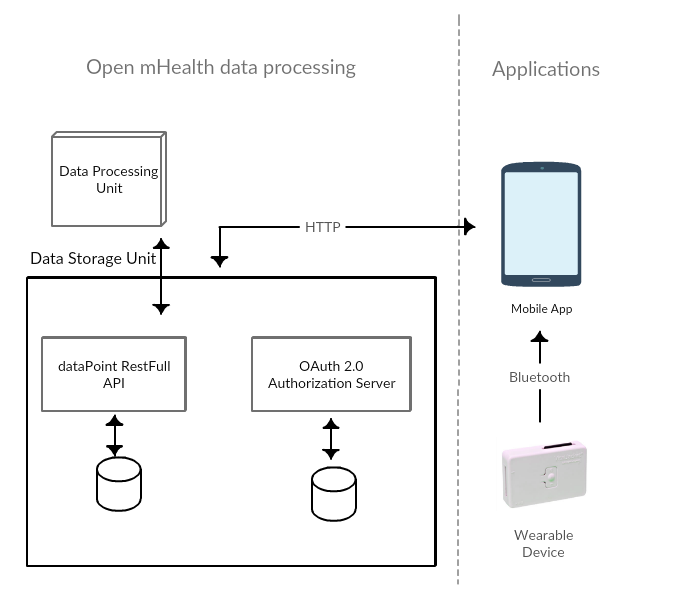
\includegraphics[width=0.9\textwidth]{imgs/omh-arch-exp.png}
  \caption[Arquitetura do caso exploratório com o Open mHealth]{Arquitetura do caso exploratório com o Open mHealth}
  
  \label{f:exp-omh-arch}
\end{figure}

\subsection{Implementação adicional}

Foi adicionado ao processo de inserção dos denominados ''dataPoint'' que é um documento que representa e deve estar em conformidade com um dos tipos de dados disponíveis denominados ''dataschemas''. Apesar dos ''dataschemas'' especificarem um formato de dados, esta validação relativa ao formato de dados não estava a ser efetuada. Um ''datapoint'' é composto por um cabeçalho onde também é definido o tipo de dados associado, e por um corpo que é formatado através do ''dataschema'' associado. Foi então feita esta validação adicional, quando o datapoint chega para ser guardado, é validado para verificar se está formatado convenientemente e só depois guardado. Esta validação é importante para posteriores consultas e tratamentos dos dados de maneira igual para cada tipo.
\par 


A \gls{OMH} tem definido um conjunto de ''data schemas'' \cite{omhschemas} que é um conjunto de esquemas de dados criados e disponíveis que especificam um formato de dados para um determinado conteúdo como por exemplo a frequência cardíaca\cite{omhschemas}. Este conjunto de schemas pode ser estendido. Ao criar um novo tipo de dados(um novo ''data schema'') podemos reutilizar outros já existentes, criando um ''data schema'' que mesmo não sendo normalizado, utiliza para definição de determinadas propriedades outros ''data schemas'' normalizados. Para experimentar esta funcionalidade foi então adicionado um novo esquema de dados para que o sistema conseguisse suportar \gls{ECG}. Esta experimentação foi conseguida com sucesso e foi uma coisa que saiu um pouco fora do cenário objetivo mas serviu para conseguir perceber muito melhor a framework. \par 

\subsection{Dificuldades e Adaptações}

As dificuldades encontradas não foram muitas, pois a framework estava bastante bem estruturada e o grau de complexidade era aceitável. As possíveis falhas desta framework era a falta de esquemas de dados para o acelerómetro, \gls{ECG} e para dados demográficos dos utilizadores da framework.

\section{Implementação exploratória: FHIR}
%http://hapifhir.io/doc_jpa.html
O \gls{FHIR} ao contrário do Open mHealth é apenas uma definição de uma \gls{API} para armazenamento de informação e troca de dados clínicos entre hospitais e clínicas. Esta \gls{API} pode ser desenvolvida de diferentes maneiras. \par 
Existe uma implementação de um projecto de código aberto com o nome Hapi-FHIR . Este projeto suporta todos os dados definidos pelo \gls{FHIR} e grande parte das operações sobre eles, como por exemplo criar, editar, eliminar, etc.
\par 
O projeto Hapi-FHIR tem um módulo denominado JPAServer  \cite{jpa-server}. Este módulo pode ser utilizado para criar um servidor FHIR, composto por uma \gls{API} \gls{REST} disponibilizando um conjunto de ''endpoints'' \gls{HTTP} para que se possa efetuar os pedidos necessários para se guardar os dados na backend. \par

\subsection{Implementação adicional}
O módulo utilizado tinha uma falha relativa à concessão de autorização sobre os pedidos efetuados, não suportando também a gestão de identidades. Para complementar este módulo foi utilizado o servidor de autorização utilizado também na experiência anterior(o servidor de autorização do \gls{DSU} do Open mHealth).
No JPAServer foi então desenvolvido um Intercetor que o que fazia, era verificar se o pedido efetuado era acompanhado por um token de acesso, caso isso acontecesse a validade do token é verificada ao servidor de autorização e então em caso de sucesso era fornecido o acesso ao pedido solicitado. Na figura \ref{f:exp-fhir-arch} temos então a arquitetura final deste caso exploratório.
\begin{figure}[H]
  \centering
  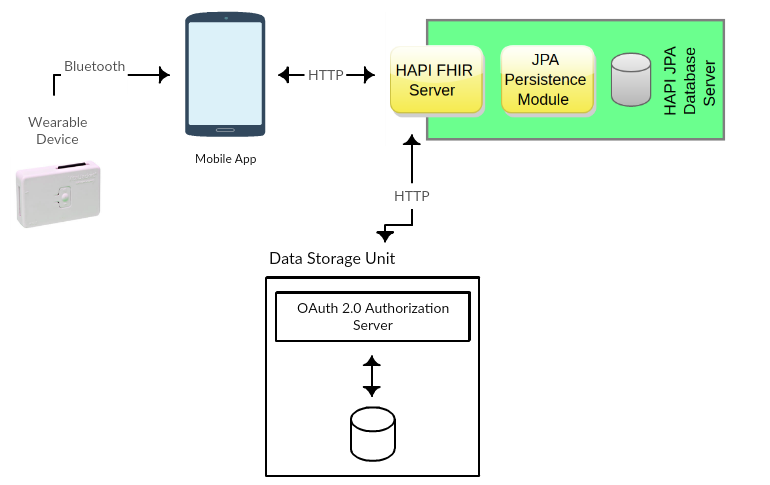
\includegraphics[width=0.9\textwidth]{imgs/fhir-arch-exp.png}
  \caption[Arquitetura do caso exploratório com o FHIR]{Arquitetura do caso exploratório com o FHIR}
  
  \label{f:exp-fhir-arch}
\end{figure}

\subsection{Dificuldades e Adaptações}
As dificuldades encontradas ainda foram algumas, neste caso temos uma definição de uma \gls{API} em vez de uma framework em si, ou seja, foram encontradas várias supostas resoluções, e no caso do Hapi-FHIR estava dividida por vários módulos, que por um lado até se pode tornar mais vantajoso porque acabamos por utilizar só aquilo que é necessário. As possíveis falhas desta \gls{API} era a falta de tipos de recursos para o acelerómetro e \gls{ECG}. Ainda temos a falta de um servidor de gestão de identidades e a concessão de autorização ao pedidos efetuados.

\section{Implementação exploratória: Google Fit}
%https://developers.google.com/fit/rest/

O Google Fit disponibiliza uma \gls{API} \gls{REST} que permite o armazenamento de dados. Esta \gls{API} permite a criação  de ''datasources''. Um ''datasource'' é criado por cada utilizador e representa  um conjunto de dados de um determinado tipo. Relativamente à concessão de acesso aos serviços \gls{REST} é utilizado o serviço de autenticação e autorização da Google baseado em OAuth 2.0. 
\par
O cenário objetivo foi desenvolvido com sucesso e na figura \ref{f:exp-googlefit-arch} podemos ver a arquitetura final deste caso exploratório.
\begin{figure}[H]
  \centering
  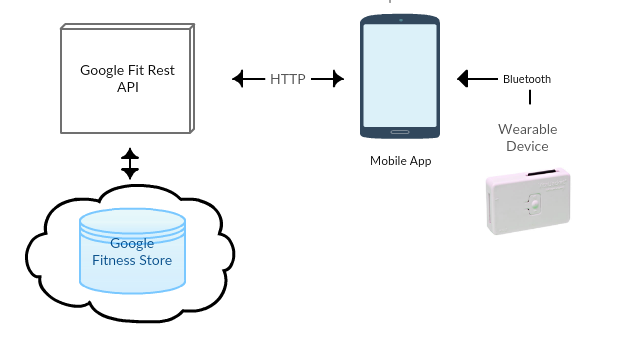
\includegraphics[width=0.9\textwidth]{imgs/googlefit-arch-exp.png}
  \caption[Arquitetura do caso exploratório com o Google Fit]{Arquitetura do caso exploratório com o Google Fit}
  
  \label{f:exp-googlefit-arch}
\end{figure}

\subsection{Dificuldades e Adaptações}

Um dos problemas encontrados nesta fase de exploração é que apesar do tipo de dados poder ser extensível, apenas era aceite dados do tipo inteiro e float, ou seja, não são suportados propriedades do tipo objeto ou array. Esta \gls{API} não tinha suporte para dados do tipo \gls{ECG}, acelerómetro e dados demográficos.

\section{Resultados e lições aprendidas}
%ico: sistematizar aquilo que foi possível concluir das implementações exploratórias discutir pontos forte / fracos observados
\subsection{Google Fit}
Começando agora pelo Google Fit, esta framework como tem como um ponto muito positivo utilizar o serviço de autenticação e autorização da Google. O primeiro ponto negativo a apontar é relativo à extensibilidade dos dados, só permitir dados do tipo inteiro e float. Para exemplificar como isto pode vir a ser um problema. No caso do \gls{ECG}, por segundo o sensor envia 500 valores, para que se possa formar um \gls{ECG} com alguma precisão. Como esta framework não suporta arrays, tinha que ser feitos 500 pedidos ao servidor por segundo para conseguir guardar e posteriormente visualizar um \gls{ECG} fidedigno. Um outro ponto negativo é o fato de esta framework ser da Google, o que isto quer dizer é que não é possível correr a framework de forma nativa e efetuar implementações extra sobre as já existentes.
\subsection{Open mHealth}
Como o \gls{OMH} é um projeto de código aberto um grande ponto forte é a possibilidade da implementação de novas funcionalidades poder ser efetuada com mais facilidade, como por exemplo a adição da validação dos dados inseridos. Tendo em conta que o projeto foi desenvolvido com o intuito de diminuir a ocorrência de formatos de dados próprios por cada aplicação no âmbito da saúde, esta pode muito bem ser uma solução para o backend do produto proposto, dado que a possibilidade da extensibilidade dos dados também é possível através da criação de novos ''data schemas'' que são posteriormente utilizados para ser efetuada a validação dos dados inseridos. 
Uma fator menos positivo é que a framework não apresenta um modelo de dados 100\% normalizado, apesar de ter sido desenvolvido com a utilização da definição da \gls{API} do \gls{FHIR}, ou seja, foi utilizado um formato normalizado para  dar suporte ao desenvolvimento deste modelo.

\subsection{FHIR}
\subsection{Análise Comparativa}
Todas as frameworks são interoperaveis (API REST)

\cleardoublepage